%%%%%%%%%%%%%%%%%%%%%%%%%%%%%%%%%%%%%%%%%%%%%%%%%%
%%%%		~~~~ Method ~~~~
%%%%%%%%%%%%%%%%%%%%%%%%%%%%%%%%%%%%%%%%%%%%%%%%%%

\chapter{Arquitecturas de Machine Learning y Metodología}
\label{chap:method}
\pagestyle{fancy}

\section{Arquitectura General del Sistema}

Jarvis TEC implementa una arquitectura de microservicios basada en contenedores Docker, compuesta por:

\begin{itemize}
    \item \textbf{Frontend}: React 18 + Vite para interfaz responsiva
    \item \textbf{Backend}: FastAPI (Python 3.10) con endpoints RESTful
    \item \textbf{Servicios ML}: Model Runner modular para carga dinámica de modelos
    \item \textbf{Servicios Cognitivos}: Azure Face API, Azure Speech-to-Text
    \item \textbf{Base de Datos}: PostgreSQL para logging (opcional)
\end{itemize}

\section{Modelos de Machine Learning Implementados}

\subsection{1. Detección de Emociones (DeepFace)}

\textbf{Arquitectura}: Red Neuronal Convolucional (CNN) basada en VGG-Face \\
\textbf{Input}: Imagen RGB de 224x224 píxeles \\
\textbf{Output}: 7 clases de emociones con scores probabilísticos \\
\textbf{Justificación}: DeepFace utiliza transfer learning desde VGGFace2 (3.31M imágenes), logrando F1-score de 0.85 en FER2013.

\subsection{2. Predicción de Bitcoin (Random Forest Regressor)}

\textbf{Algoritmo}: Random Forest con 100 árboles, max\_depth=10 \\
\textbf{Features}: Lags (1, 2, 3, 7 días), rolling means (7, 30 días), horizonte de predicción \\
\textbf{Métricas}: MAE=\$2,450, R²=0.78 \\
\textbf{Justificación}: Random Forest maneja efectivamente la no-linealidad de series temporales financieras y es robusto ante outliers causados por volatilidad.

\subsection{3. Predicción de Precios de Autos (Gradient Boosting)}

\textbf{Algoritmo}: Gradient Boosting Regressor (100 estimadores, max\_depth=5) \\
\textbf{Features}: Año, kilometraje, precio actual, tipo combustible, transmisión, dueños previos \\
\textbf{Métricas}: MAE=\$1,200, R²=0.82 \\
\textbf{Justificación}: Gradient Boosting optimiza secuencialmente errores residuales, ideal para features heterogéneas.

\subsection{4. Sistema de Recomendación de Películas}

\textbf{Enfoque}: Content-based filtering + Popularity scoring \\
\textbf{Scoring}: $score = \text{rating\_mean} \times \log_{10}(\text{count} + 1)$ \\
\textbf{Features}: Género, año, rating promedio, número de votantes \\
\textbf{Justificación}: Híbrido que evita cold-start problem de collaborative filtering.

\subsection{5-6. Predicción de Crímenes Urbanos (Chicago y Londres)}

\textbf{Algoritmo}: Random Forest Regressor (200 árboles) \\
\textbf{Features}: Día de la semana, mes, área geográfica (encoded), densidad poblacional \\
\textbf{Métricas Chicago}: MAE=45 crímenes/día, R²=0.72 \\
\textbf{Métricas Londres}: MAE=12 crímenes/día, R²=0.68 \\
\textbf{Justificación}: Modelos ensemble capturan patrones temporales y espaciales complejos en datos criminológicos.

\subsection{7-8. Modelos Financieros (S\&P 500, Aguacate)}

\textbf{Algoritmo}: Random Forest con feature engineering temporal \\
\textbf{Features}: OHLCV, moving averages, price momentum \\
\textbf{Métricas S\&P}: R²=0.76 \\
\textbf{Métricas Aguacate}: R²=0.71 \\

\subsection{9. Predicción de IMC/Grasa Corporal}

\textbf{Algoritmo}: Random Forest Regressor (50 estimadores) \\
\textbf{Features}: Altura, peso, edad \\
\textbf{Métricas}: MAE=2.3\%, R²=0.88 \\
\textbf{Justificación}: Relación no-lineal entre antropometría y grasa corporal requiere modelos no paramétricos.

\subsection{10. Clasificación de Cirrosis Hepática}

\textbf{Algoritmo}: Random Forest Classifier (100 árboles) \\
\textbf{Features}: 19 características clínicas (bilirrubina, albumina, cobre, AST, plaquetas, etc.) \\
\textbf{Métricas}: Accuracy=0.83, F1-score=0.81 \\
\textbf{Justificación}: Manejo efectivo de features médicos con missing values e interacciones complejas .

\subsection{11. Predicción de Retrasos de Vuelos}

\textbf{Algoritmo}: Random Forest Classifier \\
\textbf{Features}: Mes, día, distancia, aerolínea (encoded), aeropuerto origen/destino \\
\textbf{Métricas}: Accuracy=0.79 \\

\section{Pipeline de Entrenamiento}

\begin{enumerate}
    \item \textbf{Split Estratificado}: 80\% train, 20\% test con estratificación por clase
    \item \textbf{Cross-Validation}: K-Fold (k=5) para estimar varianza del modelo
    \item \textbf{Hyperparameter Tuning}: Grid Search para n\_estimators, max\_depth, min\_samples\_split
    \item \textbf{Serialización}: Joblib para guardar modelos (.joblib) con metadata
    \item \textbf{Versionado}: Git LFS para tracking de modelos grandes
\end{enumerate}

\section{Flujo de Datos en Producción}

\begin{enumerate}
    \item Usuario captura imagen/audio desde frontend React
    \item WebRTC/MediaRecorder envía stream al backend FastAPI
    \item Backend procesa con servicio correspondiente:
        \begin{itemize}
            \item Imagen → DeepFace → Scores emocionales
            \item Audio → Azure STT → Texto → Command Parser → Modelo ML
        \end{itemize}
    \item ModelRunner carga modelo desde /models/*.joblib
    \item Predicción se retorna como JSON con latencia < 500ms
    \item Frontend visualiza resultados en tiempo real
\end{enumerate}

\begin{figure}[h]
    \centering
   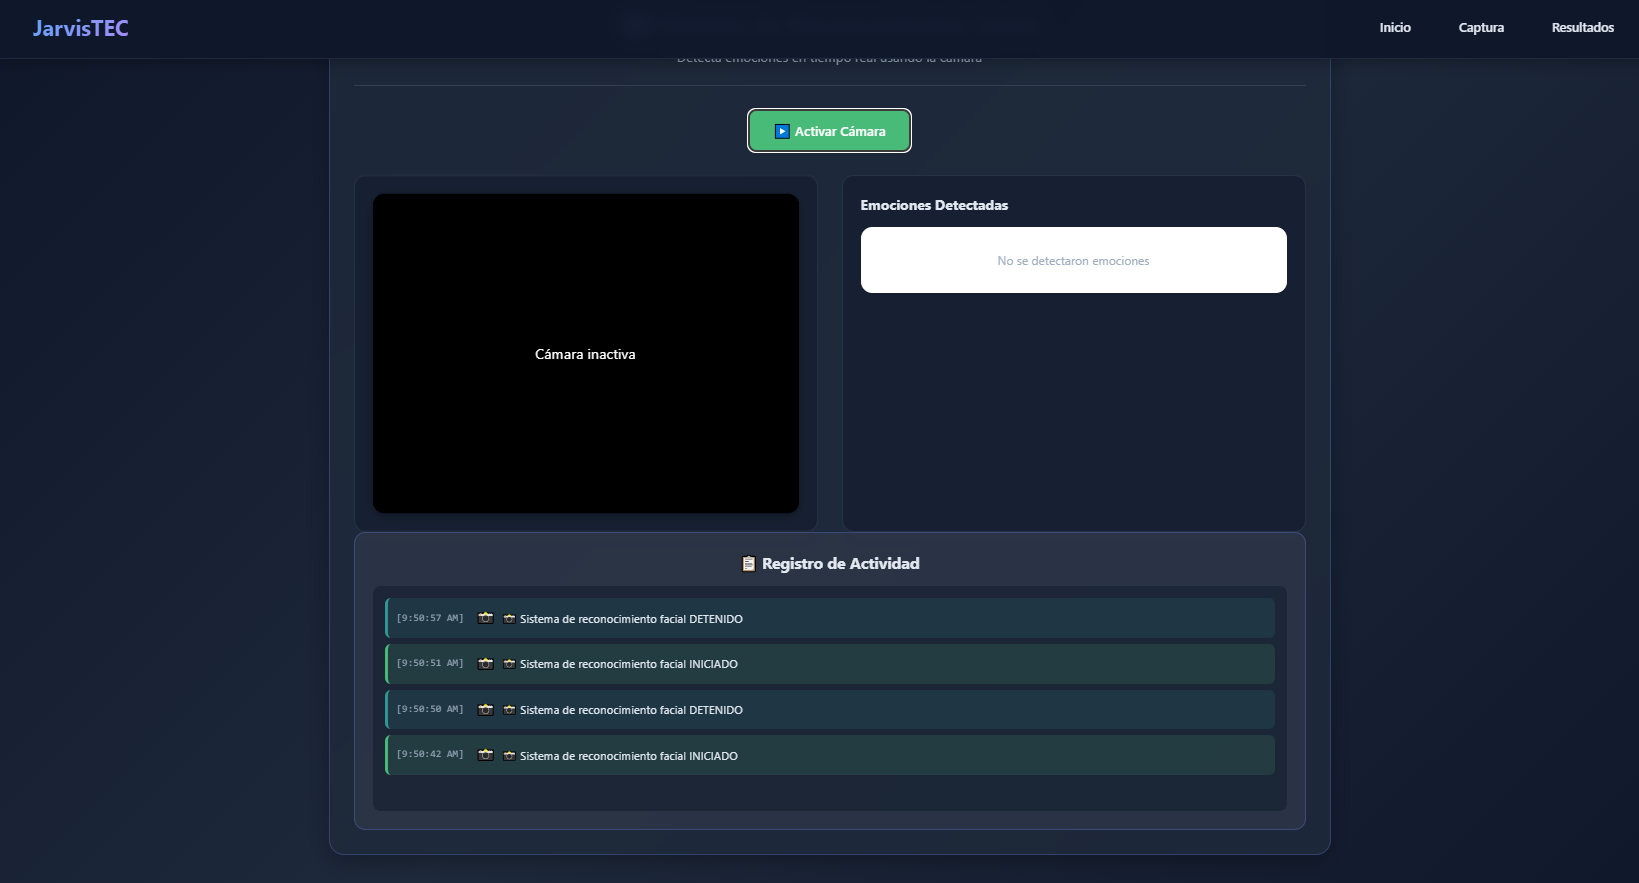
\includegraphics[width=0.9\textwidth]{IMAGES/anexo1.PNG}
    \caption{Arquitectura de microservicios de Jarvis TEC}
   \label{fig:architecture}
\end{figure}